
\section{Backend}
Após o desenvolvimento do \textit{webscraper}, foi procedido com desenvolvimento do suporte \textit{backend} do projeto.

\subsection{Organização do projeto}
Antes de iniciar a implementação definiu-se a estrutura do projeto a seguir. \textit{MVC} foi a estrutura escolhida, uma vez que, é a mais comum e bem estabelecida. Sendo assim, a organização do projeto seguiu a seguinte estrutura:
\begin{figure}[htb]
  \centering
  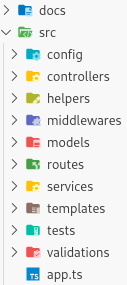
\includegraphics[width=0.2\textwidth]{images/implementacao/api/project_organization.png}
  \caption{Exemplo de página de produto incomum}
  \label{fig:63}
\end{figure}

\begin{itemize}
  \item \textbf{docs} - Documentação gerada;
  \item \textbf{src} - Base de todo o projeto;
  \item \textbf{config} - Ficheiros de configuração do projeto;
  \item \textbf{controllers} - Controladores para cada pedido;
  \item \textbf{helpers} - Ficheiros com funções gerais utilizadas regularmente;
  \item \textbf{middlewares} - Ficheiros com os middlewares da api;
  \item \textbf{models} - Classes criadas para representação de base de dados e outras entidades;
  \item \textbf{routes} - Rotas existentes;
  \item \textbf{services} - Serviços para cada pedido;
  \item \textbf{templates} - Templates de \textit{email} a serem enviados;
  \item \textbf{tests} - Testes de código realizados;
  \item \textbf{validations} - Validações a realizar do modelo de negócio e dos dados;
  \item \textbf{app} - Ficheiro de início do projeto;
\end{itemize}

\subsection{Definição de rotas base}
Após ser definida a estrutura do projeto foram estruturadas as rotas base a existir, estas referem-se a cada ator. Para uma melhor organização das rotas e da aplicação de regras, foram definidos 3 \textit{routers}, \textit{user}, para utilizadores sem sessão, \textit{professional}, para técnicos, e \textit{company} para empresas. Para indicar qual o \textit{router} a utilizar em cada pedido foi definido que:
\begin{itemize}
  \item \textbf{http://baseurl:port/professional} - Encaminhar para \textit{router} de técnicos;
  \item \textbf{http://baseurl:port/company} - Encaminhar para \textit{router} de empresas;
  \item \textbf{Restantes} - Encaminhar para \textit{router} de utilizadores;
\end{itemize}

\subsection{Middlewares} 
Um \textit{middleware} comporta-se como uma ligação entre duas partes e permite também executar código.

\subsubsection{Linguagem}
O bem essencial em uma boa comunicação entre duas partes é a utilização da mesma linguagem, pelo que, foi necessário perceber qual a linguagem a utilizar quando se responde a um pedido. Para este fim foi desenvolvido um \textit{middleware}, o objetivo deste é verificar se existe a chave \textit{language} no cabeçalho do pedido, caso esta exista é então obtida a linguagem e guardada nas variáveis locais do pedido. Na eventualidade desta não existir, foi decidido que a aplicação responderá em português por omissão, este valor poderá ser futuramente alterado de forma simples.

\newpage

\subsubsection{Autenticação}
A autenticação dos utilizadores foi implementada através de JsonWebToken, este tipo de autenticação tem por base a utilização de \textit{tokens} com tempo de expiração, o que significa que enquando o \textit{token} estiver válido, o utilizador poderá realizar pedidos e assim que este \textit{token} expirar, este terá de se autenticar novamente para obter um novo \textit{token}.
A utilização de \textit{tokens} permite também assegurar que os pedidos são realizados com \textit{tokens} gerados pela api através de uma chave de assinatura de \textit{token}, o que impede a utilização de \textit{tokens} gerados por utilizadores.
\begin{figure}[htb]
  \centering
  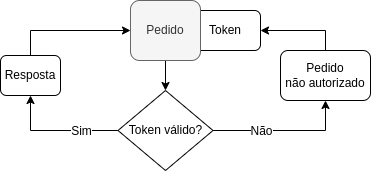
\includegraphics[width=0.5\textwidth]{images/implementacao/api/jwt_session.png}
  \caption{Utilização de tokens}
  \label{fig:64}
\end{figure}

A grande valia da utilização da técnica de autenticação mencionada anteriormente é a segurança. Isto acontece porque estes \textit{tokens} têm geralmente uma duração muito curta como por exemplo quinze minutos, e sempre que um \textit{token} de sessão expira o utilizador necessita de realizar novamente o login, o que poderá tornar a utilização da aplicação imprática.

A solução deste problema sem a perda de segurança significativa veio pelo meio da utilização de \textit{tokens} de duração maior em conjunto com os \textit{tokens} de duração curta. Enquanto o \textit{token} de grande duração se encontrar válido, novos \textit{tokens} de curta duração são gerados para o utilizador, o que leva a que o utilizador nunca perca a sua sessão. Estes \textit{tokens} de grande duração têm por nome \textit{refresh tokens} e os \textit{tokens} de curta duração têm por nome \textit{session tokens}. Sempre que o utilizador termina a sua sessão o \textit{refresh tokens} deverá ser apagado.

Sempre que um utilizador realiza um pedido,o seu \textit{token} de sessão deverá ser validado, caso este seja válido, o seu \textit{refresh token} deverá também ser validado e apenas após esta verificação o utilizador estará autenticado. Na eventualidade de o \textit{token} de sessão ou de \textit{refresh} se encontrarem expirados, este a estará sem autorização para realizar o pedido, mas poderá pedir um novo \textit{token} de sessão enquanto o seu \textit{refresh token} estiver válido, isto acontece sem realizar novamente o \textit{login} e sem o utilizador perceber.

 Além das funcionalidades atrás mencionadas é possível também associar dados em formato \textit{json} a um \textit{token jwt}, esta funcionalidade foi utilizada para enviar o \textit{id} e cargo do utilizador a qual pertence este \textit{token}.

 \newpage

\subsubsection{Validação de Papel}

Com finalidade de garantir que apenas empresas podem realizar os pedidos de empresas e apenas técnicos e empresas podem realizar os pedidos de técnicos foi então criado um middleware que valida se o utilizador que realizou o pedido tem permissões para o mesmo. Este middleware interliga-se com o middleware anterior pois como mencionado o cargo do utilizador em questão é enviado no token, sendo assim é obtido este cargo e realizada uma comparação, com o cargo desejado. Para isto foram criados 2 middlewares diferentes, um valida o cargo de empresas e o outro o cargo de técnicos. Visto que as empresas podem realizar operações de técnicos então no middleware de técnicos é verificado se o token corresponde a um utilizador empresa ou a um utilizador técnico, já no middleware de validação de empresa é verificado se o utilizador tem cargo de empresa.


% //TODO : Adicionar esquema a mostrar como estes middlewares funcionam


\subsection{Logging de erros}

A identificação dos erros no servidor é difícil, pois, uma vez que os erros são tratados, os dados referentes aos não são guardados ou utilizados. Para resolver este problema foi decidido que sempre que um erro que não é customizado é detetado, é registado um \textit{log}, este contém informações sobre o pedido como data e hora, dados recebidos, a descrição original do erro e serviço referente.

Para implementar esta solução foi em primeiro lugar criado um \textit{middleware} que sempre que deteta erros dentro do serviço executa um método. Este método, por sua vez, obtém os dados referentes ao pedido realizado, sendo estes a data e hora, os dados recebidos e o serviço pedido. Após se obter os dados do pedido é obtida a mensagem do erro e estes dados acrescentados numa nova linha no ficheiro de erros do servidor.

\subsection{Logging de pedidos com morgan}

Para realizar o \textit{logging} de pedidos a serviços foi utilizado o \textit{morgan}, esta ferramenta apenas precisa a indicação do ficheiro onde escrever os \textit{logs}, o que leva à utilização de um ficheiro chamado \textit{log}. O \textit{morgan} também precisa da indicação do tipo de \textit{log} a realizar, estes tipos são indicados pela ferramenta, o utilizado foi o combinado, este é o tipo de \textit{log} mais completo, visto que, é o que obtém mais dados, sendo estes, a data e hora do pedido, o tipo de pedido, o serviço pedido, os dados recebidos, a resposta devolvida e também a descrição do sistema utilizado.

\subsection{Controllers}
Assim que um pedido consegue ultrapassar todos os \textit{middlewares} sem ser impedido, este é então redirecionado para um \textit{controller}.

\subsubsection{Estruturação dos controllers}
Para evitar variação de código destes \textit{controllers} em termos de estrutura, foi então decidido desenhar uma estrutura de \textit{controller} e aplicar esta perante o demais código. Esta segue as seguintes etapas:
\begin{enumerate}
 \item Obter dados do pedido
 \item Validar se os dados obrigatórios são obtidos
 \item Validar o pedido perante o modelo de negócio
 \item Executar a lógica do pedido
 \item Formular a resposta e enviar
 \item Em caso de erro este deverá ser capturado e processado para enviar um erro para o utilizador
\end{enumerate}

 Esta estrutura será sempre aplicada pois foram utilizados \textit{snippets} de código que permitem criar um modelo de estrutura sendo apenas necessário escrever a palavra-chave e toda a estrutura é aplicar, pelo que é necessário de seguida efetuar as alterações perante o contexto.

\newpage

\subsubsection{Execução da lógica de negócio}
A execução da lógica de negócio passa por direcionar os dados para a ação correta, esta ação geralmente resulta numa operação de base de dados. Inicialmente foi desenvolvida toda a validação de código e todas as operações de base de dados diretamente na execução da lógica de negócio. Após uma revisão desta organização de código com o professor orientador, foi decidido separar estas funcionalidades, de onde surgiu a componente de validação de dados, a de operações de base de dados e a de lógica de negócio que implementa a componente de operações de base de dados. Sendo assim para evitar que estas operações sobre a base de dados estejam em conjunto com o direcionamento dos dados, foram criados modelos para cada tabela. Cada modelo contém um conjunto de operações sobre a tabela correspondente. Estas operações estão contidas sobre métodos que podem receber dados para executar na operação e devolver a resposta da mesma.

\subsubsection{Validação dos dados}
A validação dos dados é necessária para evitar erros a nível de servidor com dados em falta e também para aplicar as regras de negócio. Para realizar estas validações é em primeiro lugar verificado se todos os dados são recebidos, de seguida estes são enviados para um validador. O validador executa todas as verificações necessárias a nível de regras de negócio e na possibilidade de alguma regra não ser cumprida, é então atirado um erro.

\subsubsection{Formulação da resposta}
Assim como mencionado anteriormente o bem mais importante numa boa comunicação é a utilização da mesma linguagem, pelo que a resposta do servidor deverá  utilizar a linguagem indicada pelo utilizador. Para realizar esta tradução foi utilizado o mesmo conceito que se usa em \textit{android}. Neste é criado um ficheiro que contém um conjunto de chaves e a cada corresponde um texto. Cada tradução tem de conter estas chaves para ser possível obter o texto correto para cada chave. Sendo assim foi utilizado um ficheiro \textit{json} que contem as chaves das linguagens suportadas, a cada uma corresponde a um conjunto de outras chaves que contém todas as traduções necessárias, neste caso foi utilizado numeração, em vez de palavras. Esta abordagem permite que de forma fácil futuramente seja possível adicionar outras linguagens ao servidor.

\begin{figure}[htb]%
  \centering
  \subfloat[\centering Página de login]{{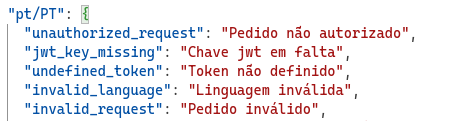
\includegraphics[width=0.45\textwidth]{images/implementacao/api/trad_pt.png} }}%
  \qquad
  \subfloat[\centering Página de registo]{{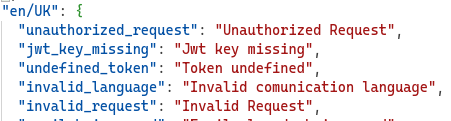
\includegraphics[width=0.45\textwidth]{images/implementacao/api/trad_en.png} }}%
  \caption{Autenticação - Login e Registo}%
  \label{fig:24}
\end{figure}

O suporte a este ficheiro foi elaborado com uma operação que recebe a chave e a linguagem desejada. Este devolve o texto correspondente traduzido, pelo que na formulação da resposta a operação é executada com a indicação da chave do texto a enviar e a linguagem desejada, sendo então este devolvido para o utilizador.

\newpage

\subsubsection{Processamento de erros}
Como não é de interesse enviar erros do próprio servidor para o utilizador, foi decidido controlar estes. Para isso foi criado um erro customizado com base o erro da própria linguagem. Este recebe por parâmetro o código da tradução da mensagem. Esta abordagem permite também evitar que sempre que um erro é lançado o sistema pare. Sempre que um erro é lançado por base de dados, erro de código ou de biblioteca, o erro original é chamado, pelo que foi decidido que sempre que é detetado, então será devolvida uma mensagem de "erro de servidor" o que evita que dados sensíveis e desnecessários para o utilizador sejam devolvidos.

\subsection{Envio de \textit{emails}}
Como mencionado no capítulo \ref{sec:emails_send}, não é permitido a utilização de acentuação na escrita de \textit{emails} no \textit{Tabular}, pelo que, primeiramente todos os problemas foram resolvidos. Para permitir que os dados dos \textit{emails} sejam personalizaveis, como por exemplo, dados de utilizador e \textit{link} para clicar, estes \textit{emails} são colocados em métodos que recebem por parâmetro os dados para serem colocados dentro do \textit{html} do \textit{email}, este método, por fim, devolve em \textit{string} o conteúdo a enviar.

Para o envio de \textit{emails} é necessário um servidor e um serviço de envio. Para vias de teste foi utilizado um servidor gratuito de \textit{email} hospedado por \textit{Mailjet}. Após a fase de testes foi alterado para o servidor de \textit{email} da empresa, o que permitiu que seja identificado como empresa Motorline.

O serviço de envio de \textit{emails} foi utilizado o \textit{Nodemailer}. A configuração do servidor de \textit{emails} do \textit{Nodemailer} é realizada através de uma chamada ao objeto do servidor com a indicação das configurações que estão no ficheiro \textit{.env}. Esta chamada ao servidor, por sua vez, devolve um objeto que fornece métodos para enviar \textit{emails}, sendo este, criado e utilizado sempre que se deseja enviar \textit{emails} no servidor.

Para evitar que sempre que se deseja enviar um \textit{email} seja necessário indicar todos os dados de configuração do servidor, foi elaborado um método que cria e devolve o objeto do servidor sempre que necessário. Sendo assim, sempre que se deseja enviar um \textit{email} é primeiramente obtido o objeto do servidor, de seguida é invocado o método para obter o conteúdo \textit{html} do \textit{email} e por fim, é utilizado o objeto do servidor para chamar o método de envio de \textit{emails}, no qual, se terá de indicar o \textit{email} do destinatário, o assunto e o conteúdo.


\newpage



\subsection{Agendamento de tarefas}

Com a utilização da ferramenta \textit{node-cron} foi inicialmente programado para enviar o relatório de notificações todos os dias às 22 horas. Esta configuração foi relizada através da indicação da programação de horário de envio, para isso é utilizada a estrutura segundo, minuto, hora, dia do mês, mês, dia da semana. Como o objetivo é as 22 horas, os segundos e minutos foram indicados como 0 e as horas foram indicadas como 22, já o restante foi indicado com o símbolo "*" que indica que o processo deverá occorrer em todas as instâncias dos restantes valores, o que significa todos os dias. A configuração final obtida foi "0 0 22 * * *".

Quando o método do agendamento é invocado, são obtidos todos os utilizadores com a configuração de relatório de notificações ativa, em primeiro lugar, para cada um destes, são obtidas todas as notificações do dia. De seguida é criado o objeto de servidor e invocado o método para obter o conteúdo de notificações através da indicação todas as notificações do utilizador. Por fim, é enviado o \textit{email} para o utilizador com todas as suas notificações e um \textit{link} para aceder rápidamente ao ecrã de notificações.



\newpage

\input{sections/chap4/2.servicos_backend/9.segurança.tex}

\subsection{Documentação Typedoc}
Durante a implementação do typedoc foi detetado que a categorização de documentação não se encontrava funcional devido a um problema encontrado pelos desenvolvedores da ferramenta. Foi decidido então reduzir a versão para uma com a funcionalidade ativa, mas esta não se encontrava compatível com a versão mais atualizada de \textit{typescript}, pelo que não foi possível explorar esta funcionalidade. Para contornar o problema foi decidido explorar outra funcionalidade menos utilizada, esta permite converter qualquer documentação em módulos, estes podem então ser categorizados, o problema é que é criado um modelo genérico do código o qual não permite a fácil identificação das tipagens de \textit{scripts}. Estes módulos permitem também a categorização dos mesmos, o que permite um nível de organização da documentação gerada maior.

\begin{figure}[htb]
  \centering
  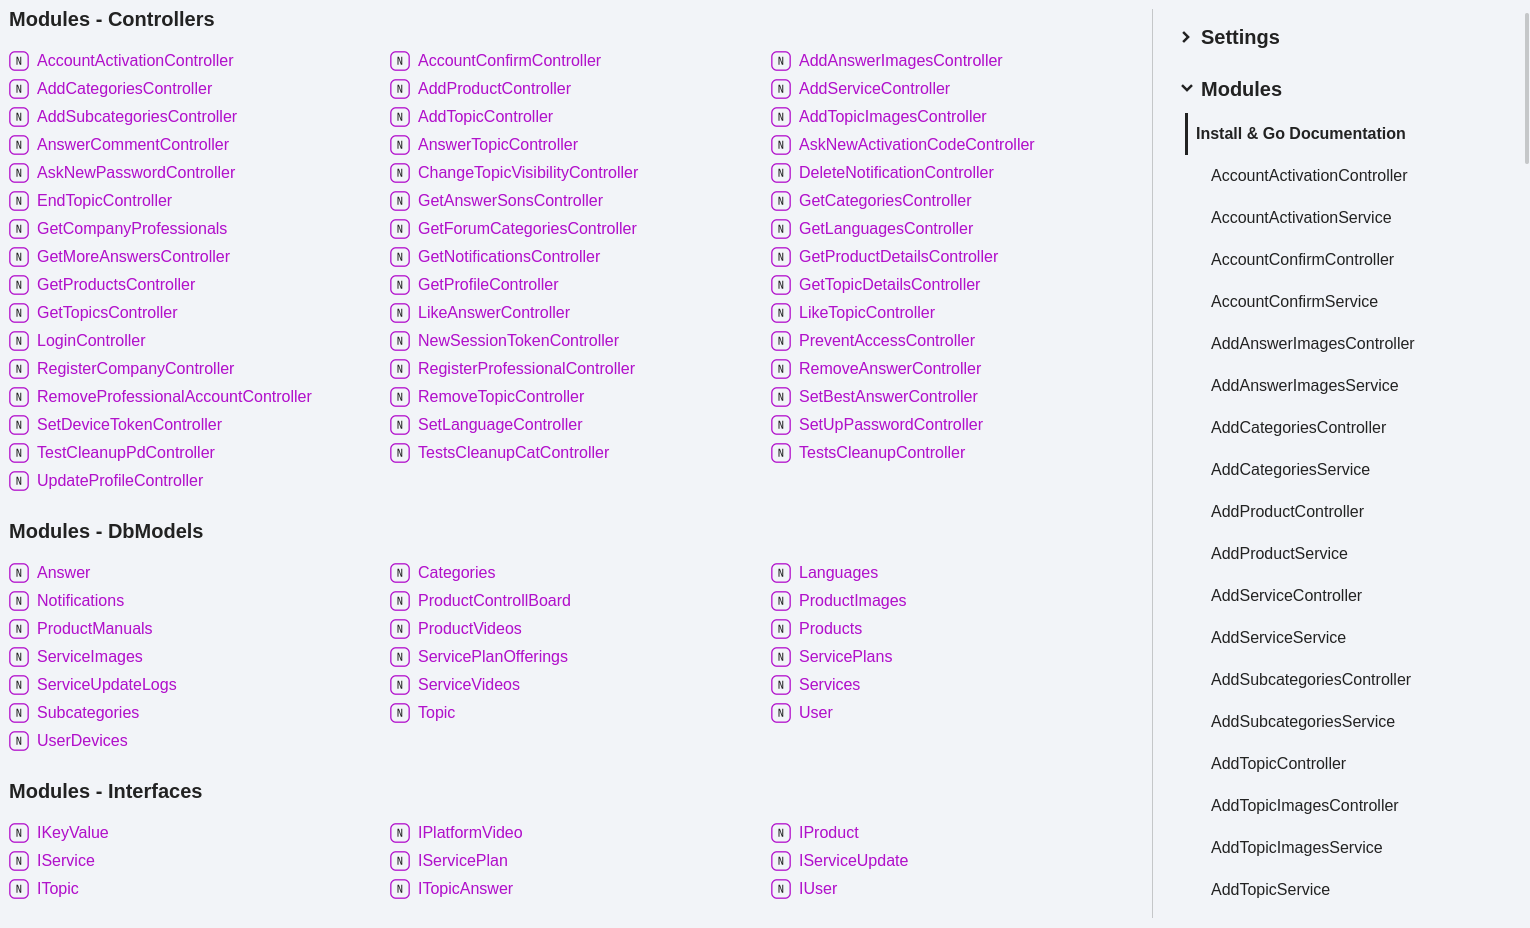
\includegraphics[width=0.5\textwidth]{images/implementacao/api/docs.png}
  \caption{Documentação \textit{typedoc}}
  \label{type_doc}
\end{figure}

\newpage

\subsection{Documentação Swagger}
Apesar do swagger ferramenta disponibilizar a funcionalidade de gerar automáticamente documentação a partir de comentários de código, foram encontrados alguns problemas com esta funcionalidade, o que levou a que não fosse possível não gerar a documentação. Visto isto, foi optado por manter a documentação manualmente com o ficheiro \textit{json}. Esta ferramenta oferece diversas funcionalidades como autenticação, definição de estruturas de dados para os serviços e exemplos de respostas, ambas estas funcionalidades foram exploradas o que permitiu um bom suporte de documentação para qualquer utilizador.

\begin{figure}[htb]
  \centering
  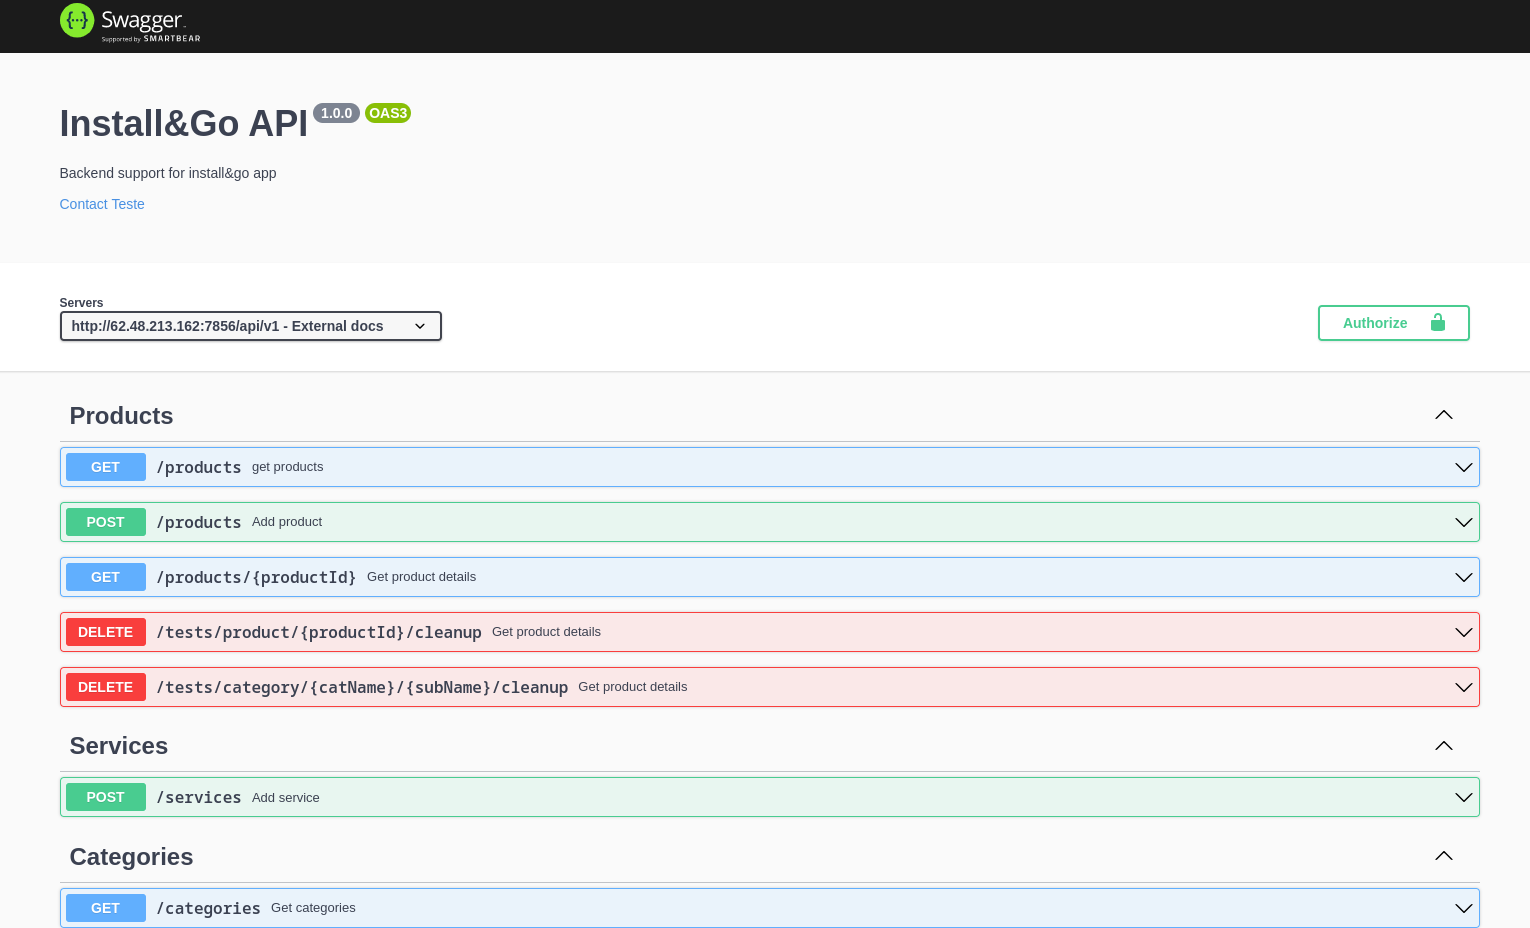
\includegraphics[width=0.6\textwidth]{images/implementacao/api/swagger_intro.png}
  \caption{Documentação swagger}
  \label{fig:67}
\end{figure}

\begin{figure}[htb]
  \centering
  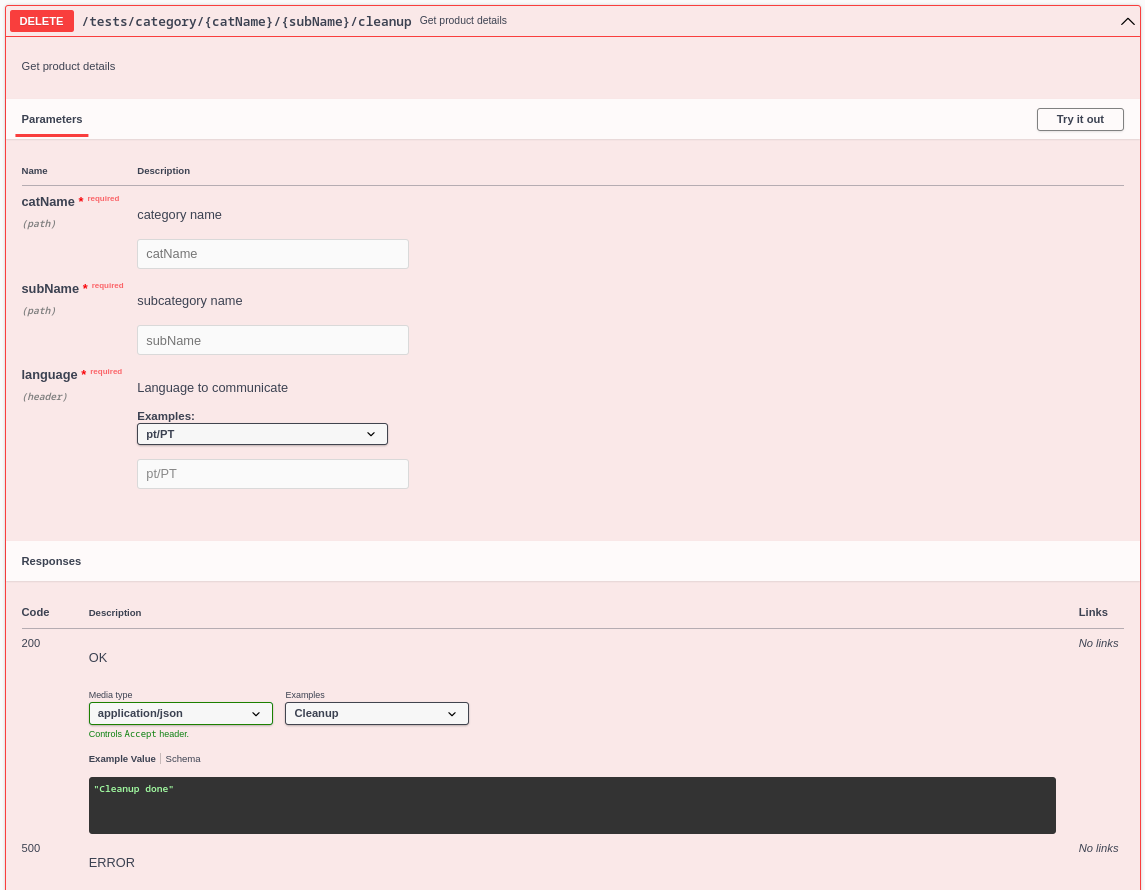
\includegraphics[width=0.6\textwidth]{images/implementacao/api/swagger_pedido.png}
  \caption{Exemplo de documentação de serviço}
  \label{fig:68}
\end{figure}
